\section{Discussion}\label{sec:discussion}

\texttt{ct-verif} operates at the level of LLVM bitcode and can therefore only formally attest to whether a program's
representation as bitcode is constant-time.

Translating a bitcode program into binary is a straightforward process and is generally a simple one-to-one mapping between bitcode instructions and assembly.
In theory an assembly program should therefore preserve the constant-time property if the source LLVM bitcode is proven to be constant-time.

However, while this argument does hold for simple RISC-like ISAs, it does not for complex CISC-like machines like the x86 architecture.
There is in reality no true ``x86'' machine as no x86 processor actually executes the CISC instructions it receives as input directly.
Instead, these CISC instructions are decomposed into RISC-like $\mu$Ops before being scheduled for execution on a RISC-like backend.
This decomposition is handled transparently by microcode sequencers in the CPU's frontend and is not under the control of the user as microcode updates can change instruction behavior.
Asserting that a constant-time LLVM bitcode program remains constant-time when translated to x86 assembly is unclear as users have no way of knowing how an instruction is decoded into $\mu$Ops.

The \texttt{dudect} project appeared after \texttt{ct-verif} and suggested the only way to decide whether a program is constant-time or not is to actually run it and time its execution~\cite{dudect}.
The main idea behind \texttt{dudect} is to run a supposedly constant-time program under two environments and measure its execution time: (1) using \textcolor{red}{fixed} secret inputs, and (2) using \textcolor{blue}{random} secret inputs.
If the program is constant-time, then the timing traces of these two programs should be indistinguishable.
However, machines do not have deterministic execution times due to caches and OS scheduling, so relying on the execution time alone to determine constant-timeness would be incorrect.
\texttt{dudect} therefore proposes using a statistical method---an ``equivalence of means'' $t$-test---to determine whether multiple program executions under the two aforementioned environments are statistically indistinguishable.
If yes, then the program is \emph{possibly} constant-time. If not, then the program is \emph{definitely not} constant-time.
Combined with a formal constant-time proof obtained from \texttt{ct-verif}, the mechanism proposed by \texttt{dudect} can validate that the $\mu$Op decomposition of a program is constant-time.

We evaluated the \texttt{dudect} method on 9 examples from the \texttt{ct-verif} paper and were able to validate their constant-time property.
In fact, \texttt{dudect}'s method of operation lends itself well to a graphical validation when a constant-time violation is detected.
Indeed, repetitively running the program with fixed/random private inputs and plotting the CDF of its average execution time generates curves that should perfectly overlap if the program is constant-time\footnote{We modified \texttt{dudect} to automatically extract and plot its timing information.}.
Figure~\ref{fig:dudect_donna} shows an example of running the \texttt{dudect} method on two implementations of \texttt{curve25519} that differ in the constant-time property.

\begin{figure}[h!]
  \centering
  \subfigure[Non-CT implementation]{
      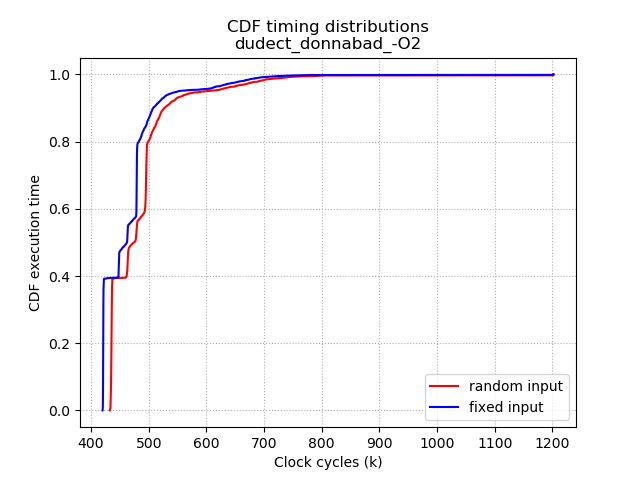
\includegraphics[width=0.45\textwidth]{./figs/donnabad_cdf.png}
  }\label{fig:dudect_donnabad}
  \subfigure[CT implementation] {
      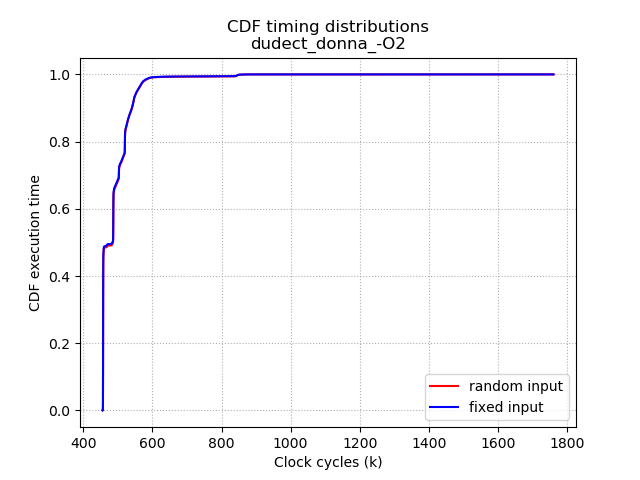
\includegraphics[width=0.45\textwidth]{./figs/donnagood_cdf.png}
  }\label{fig:dudect_donnagood}
  \caption{CDF timing behavior of a non-CT vs CT implementation of an elliptic curve.}
  \label{fig:dudect_donna}
\end{figure}

Figure~\ref{fig:dudect_sha} in turn shows how an example that a formal tool could not prove as constant-time \emph{could} be constant-time since the execution curves overlap perfectly.

\begin{figure}[h!]
  \centering
  \subfigure[SHA256]{
      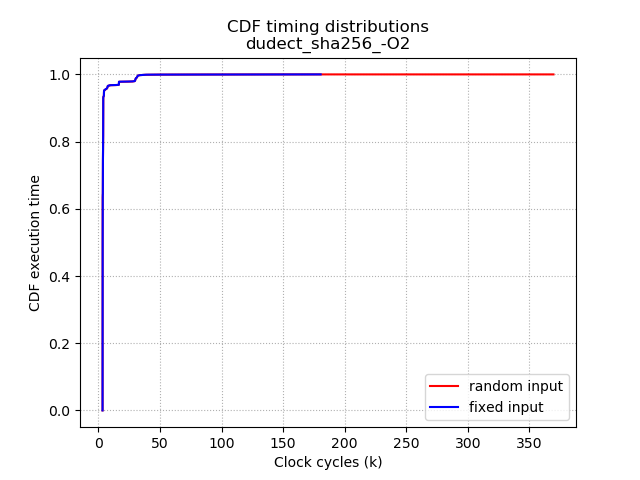
\includegraphics[width=0.45\textwidth]{./figs/sha256_cdf.png}
  }\label{fig:dudect_sha256}
  \subfigure[SHA512] {
      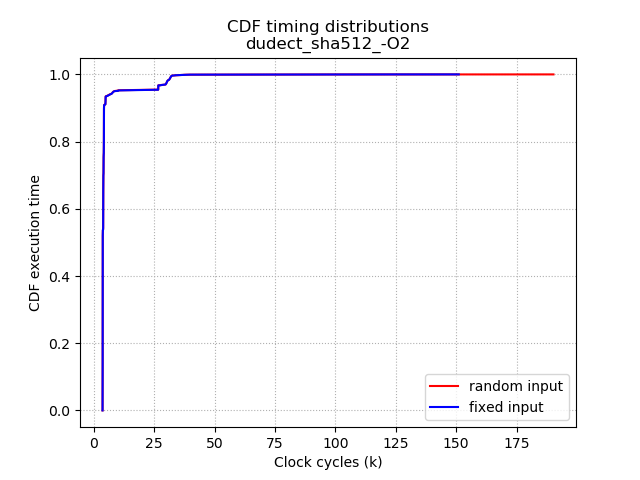
\includegraphics[width=0.45\textwidth]{./figs/sha512_cdf.png}
  }\label{fig:dudect_sha512}
  \caption{CDF timing behavior of \texttt{libsodium}'s SHA256/SHA512 implemenation. Both are statistically constant-time.}
  \label{fig:dudect_sha}
\end{figure}

% The \texttt{ct-verif} tool was released in 2016, two years before widespread micro-architectural side-channel attacks like Meltdown~\cite{meltdown} and Spectre~\cite{spectre} were reported.
% Formal techniques are, in theory, able to detect whether a program is vulnerable to certain categories of side-channel attacks.
% A program's constant-timeness property can be formally verified, but only if one assumes the program model is correct.
% Indeed \texttt{ct-verif} uses LLVM's operation cost model to determine whether an instruction
% The disclosure of such attacks encourages the use of formal techniques to verify a design's implementation
